%%%%%%%%%%%%%%%%%%%%%%%%%%%%%%%%%%%%%%%%%
% Masters/Doctoral Thesis 
% LaTeX Template
% Version 2.4.1 (20/05/17)
%
% University of Applied Sciences
% Department of Computer Science 
% ---------------------------------------
% B.Sc. & M.Sc. Thesis Template
% Template modified by Stephan Gimbel
% Contact: stephan.gimbel@h-da.de
% Web: https://www.fbi.h-da.de/organisation/personen/gimbel-stephan.html
% ---------------------------------------
%
% Original Template Information:
%
% This template has been downloaded from:
% http://www.LaTeXTemplates.com
%
% Version 2.x major modifications by:
% Vel (vel@latextemplates.com)
%
% This template is based on a template by:
% Steve Gunn (http://users.ecs.soton.ac.uk/srg/softwaretools/document/templates/)
% Sunil Patel (http://www.sunilpatel.co.uk/thesis-template/)
%
% Template license:
% CC BY-NC-SA 3.0 (http://creativecommons.org/licenses/by-nc-sa/3.0/)
%
%%%%%%%%%%%%%%%%%%%%%%%%%%%%%%%%%%%%%%%%%

%----------------------------------------------------------------------------------------
%	PACKAGES AND OTHER DOCUMENT CONFIGURATIONS
%----------------------------------------------------------------------------------------

\documentclass[
11pt, % The default document font size, options: 10pt, 11pt, 12pt
%oneside, % Two side (alternating margins) for binding by default, uncomment to switch to one side
%english, % ngerman for German
english,
singlespacing, % Single line spacing, alternatives: onehalfspacing or doublespacing
%draft, % Uncomment to enable draft mode (no pictures, no links, overfull hboxes indicated)
%nolistspacing, % If the document is onehalfspacing or doublespacing, uncomment this to set spacing in lists to single
%liststotoc, % Uncomment to add the list of figures/tables/etc to the table of contents
%toctotoc, % Uncomment to add the main table of contents to the table of contents
%parskip, % Uncomment to add space between paragraphs
%nohyperref, % Uncomment to not load the hyperref package
%headsepline, % Uncomment to get a line under the header
%chapterinoneline, % Uncomment to place the chapter title next to the number on one line
%consistentlayout, % Uncomment to change the layout of the declaration, abstract and acknowledgements pages to match the default layout	
]{MastersDoctoralThesis} % The class file specifying the document structure
\usepackage[utf8]{inputenc} % Required for inputting international characters
\usepackage[T1]{fontenc} % Output font encoding for international characters
\usepackage{palatino} % Use the Palatino font by default
\usepackage{siunitx} % Added package to display units
\usepackage{mathrsfs}
\usepackage{amssymb}
\usepackage{amsmath}
\usepackage{float}
\usepackage{subfigure}
\usepackage{framed}
\usepackage{xcolor}
\usepackage{xspace}
\usepackage{hyperref}
\usepackage{graphicx}
\usepackage{tabularx}
\usepackage{enumitem}
%\usepackage{abntcite}
\usepackage[backend=biber,style=alphabetic,natbib=true]{biblatex} % Use the bibtex backend with the authoryear citation style (which resembles APA)
% possible styles: numeric, alphabetic, authoryear, authortitle, verbose, reading, draft
\addbibresource{library.bib} % The filename of the bibliography
\usepackage{filecontents}
\usepackage[autostyle=true]{csquotes} % Required to generate language-dependent quotes in the bibliography

%----------------------------------------------------------------------------------------
%	MARGIN SETTINGS
%----------------------------------------------------------------------------------------

\geometry{
	paper=a4paper, % Change to letterpaper for US letter
	inner=2.5cm, % Inner margin
	outer=3.8cm, % Outer margin
	bindingoffset=.5cm, % Binding offset
	top=1.5cm, % Top margin
	bottom=1.5cm, % Bottom margin
	%showframe, % Uncomment to show how the type block is set on the page
}

%----------------------------------------------------------------------------------------
%	THESIS INFORMATION
%----------------------------------------------------------------------------------------

\thesistitle{Data-driven process discovery} % Your thesis title, this is used in the title and abstract, print it elsewhere with \ttitle
\supervisor{Prof. Dr. Markus D\"ohring} % Your supervisor's name, this is used in the title page, print it elsewhere with \supname
%\supervisor{Prof. Dr. Brian S. \textsc{Smith}}
\examiner{Prof. Dr. Markus D\"ohring} % Your examiner's name, print it elsewhere with \examname
%\examiner{Prof. Dr. Sangeeta \textsc{Singh}}
\degree{Master of Science (M.Sc.)} % Your degree name, print it elsewhere with \degreename
%\degree{Master of Science (M.Sc.)}
%\author{John \textsc{Smith}} % Your name, print it elsewhere with \authorname
\author{Lisa Stolz}
\addresses{} % Your address, this is not currently used anywhere in the template, print it elsewhere with \addressname

\subject{Data science} % Your subject area, this is not currently used anywhere in the template, print it elsewhere with \subjectname
\keywords{} % Keywords for your thesis, this is not currently used anywhere in the template, print it elsewhere with \keywordnames
%\university{\href{http://www.university.com}{Hochschule Darmstadt}} % Your university's name and URL, this is used in the title page and abstract, print it elsewhere with \univname
%\university{\href{http://www.h-da.de}{Hochschule Darmstadt}} % Your university's name and URL, this is used in the title page and abstract, print it elsewhere with \univname
\university{{Hochschule Darmstadt}} % Your university's name and URL, this is used in the title page and abstract, print 
%\department{\href{http://fbi.h-da.de}{Fachbereich Informatik}} % Your department's name and URL, this is used in the title page and abstract, print it elsewhere with \deptname
\department{{Fachbereich Mathematik}}
\group{\href{http://researchgroup.university.com}{Research Group Name}} % Your research group's name and URL, this is used in the title page, print it elsewhere with \groupname
\faculty{\href{http://faculty.university.com}{Faculty Name}} % Your faculty's name and URL, this is used in the title page and abstract, print it elsewhere with \facname

\AtBeginDocument{
%\hypersetup{pdftitle=\thesistitle} % Set the PDF's title to your title
%\hypersetup{pdfauthor=\author} % Set the PDF's author to your name
%\hypersetup{pdfkeywords=\keywords} % Set the PDF's keywords to your keywords
}

\begin{document}

\frontmatter % Use roman page numbering style (i, ii, iii, iv...) for the pre-content pages

\pagestyle{plain} % Default to the plain heading style until the thesis style is called for the body content

%----------------------------------------------------------------------------------------
%	TITLE PAGE
%----------------------------------------------------------------------------------------

\begin{titlepage}
\begin{center}

\vspace*{.06\textheight}

\includegraphics[width=8cm]{Logo/logo_h_da_fbmn300.png}
\vspace*{.02\textheight}

\Large{\textbf{\textsf{Hochschule Darmstadt}}} \\
\Large{\textsf{- Fachbereich Mathematik -}}
\vspace*{.06\textheight}
 
\huge{\textbf{\textsf{\ttitle}}}\\
\vspace{0.5em}
\Large{\textbf{\textsf{Reproduktion und kritische Betrachtung der Ergebnisse von F. Mannhardt et al.(TU/e)}}} \\
 
\vspace{3em}

\large{\textsf{Abschlussarbeit im Hauptseminar - Hot Topics in Data Science}} \\ \vspace{0.5em}
%\Large{\textbf{\textsf{\degreename}}} \\ \vspace{0.5em}
\large{\textsf{vorgelegt von}}
 
\vspace*{.04\textheight}
 
\textsf{\authorname}
 
\vspace{4.0em}

\begin{spacing}{1.5}
\textsf{\makebox[3.5cm][l]{Referent:}}            \textsf{\makebox[7cm][r]{\supname}} \\
\textsf{\makebox[3.5cm][l]{Korreferentin:}}           \textsf{\makebox[7cm][r]{\examname}} \\
\textsf{\small{\makebox[3.5cm][l]{Ausgabedatum:}}}  \textsf{\small{\makebox[7cm][r]{\today}}} \\
\textsf{\small{\makebox[3.5cm][l]{Abgabedatum:}}}   \textsf{\small{\makebox[7cm][r]{\today}}}
\end{spacing}

\end{center}
\end{titlepage}
\newpage
%----------------------------------------------------------------------------------------
%	DECLARATION PAGE
%----------------------------------------------------------------------------------------

\begin{declaration}
\addchaptertocentry{\authorshipname} % Add the declaration to the table of contents
\noindent Ich, \authorname, versichere hiermit, dass ich die vorliegende Arbeit selbstständig verfasst und keine anderen als die im Literaturverzeichnis angegebenen Quellen benutzt habe. \\ 

\noindent Alle Stellen, die wörtlich oder sinngemäß aus veröffentlichten oder noch nicht veröffentlichten Quellen entnommen sind, sind als solche kenntlich gemacht.\\

\noindent Die Zeichnungen oder Abbildungen in dieser Arbeit sind von mir selbst erstellt worden oder mit einem entsprechenden Quellennachweis versehen. Diese Arbeit ist in gleicher oder ähnlicher Form noch bei keiner anderen Prüfungsbehörde eingereicht worden.\\

\noindent Darmstadt, den \today

\vspace{5em}
\noindent\rule[1em]{25em}{0.5pt}\\ % This prints a line for the signature
(Vollständige, handschriftliche Unterschrift)

\end{declaration}

\cleardoublepage

%----------------------------------------------------------------------------------------
%	ABSTRACT PAGE
%----------------------------------------------------------------------------------------
\begin{abstract}
\addchaptertocentry{\abstractname} % Add the abstract to the table of contents
\vspace{3em}
Ziel dieser Seminararbeit ist die kritische Auseinandersetzung mit dem Paper "Data-driven process discovery: revealing conditional
infrequent behavior from event logs\grqq{} \\ von F. Mannhardt et. al. der Technischen Univerität Eindhoven.\\
Die Autoren stellen in dieser Arbeit den \glqq Data-aware Heuristic Miner\grqq{} (DHM) vor, welcher bisherige heuristische Process Mining Ansätze um ein Maß der bedingten Abhängigkeit erweitert.\\
Der DHM basiert auf der Idee, dass seltenes - jedoch durch Daten gestütztes - Prozessverhalten nicht als Hintergrundrauschen verworfen werden sollte.
Die Autoren erklären in ihrer Arbeit zunächst die theoretischen Hintergründe des DHM und zeigen anschließend die Ergebnisse der Evaluierung in ProM.\\
\vspace{0.5em}

In dieser Arbeit wird zunächst ein kurzer Überblick über den DHM und die Erweiterung bisheriger heuristischer Ansätze des Process Mining gegeben.\footcite{Mannhardt17}
Der Schwerpunkt liegt anschließend auf der praktischen Anwendung des Pakets \glqq DataAwareCNetMiner\grqq{} in ProM, einem interaktiven Tool, das einen schnellen Vergleich mit dem \glqq standard Flexible Heuristic Miner\grqq{} erlaubt.\\
Zunächst werden die im Paper dargestellten Evaluierungen reproduziert und getestet ob die Ergebnisse nachvollzogen werden können.\\
Die erste Evaluierung basiert auf einem synthetisch generierten Datensatz und die zweite auf realen Event Logs zu Strafzetteln im italienischen Straßenverkehr und Krankenhausrechnungen eines Enterprise Resource Planing Tools.\\
Wenn die Ergebnisse und das Vorgehen der Autoren reproduziert werden können, werden im Anschluss die Versuchsparameter variiert (z.B. Klassifizierung durch Entscheidungsbäume C3.4 und Objektivitätsmaß Cohens Kappa).
Schließlich werden die bis dahin getesteten Mining Methoden auf einen neuen Eventlog Datensatz angewendet und mit den bisherigen Ergebnissen verglichen.


\end{abstract}


%----------------------------------------------------------------------------------------
%	LIST OF CONTENTS/FIGURES/TABLES PAGES
%----------------------------------------------------------------------------------------

\tableofcontents % Prints the main table of contents

\listoffigures % Prints the list of figures

\listoftables % Prints the list of tables

%----------------------------------------------------------------------------------------
%	ABBREVIATIONS
%----------------------------------------------------------------------------------------

\begin{abbreviations}{ll} % Include a list of abbreviations (a table of two columns)


\textbf{DHM} & \textbf{D}ata-aware \textbf{H}euristic \textbf{M}iner\\
\textbf{HM} & \textbf{H}euristic \textbf{M}iner\\
\textbf{IM} & \textbf{I}nductive \textbf{M}iner\\


\end{abbreviations}


%----------------------------------------------------------------------------------------
%	SYMBOLS
%----------------------------------------------------------------------------------------

\begin{symbols}{lll} % Include a list of Symbols (a three column table)

$C = (\Sigma, s_i , s_o , D, I, O)$ & Causal nets (C-nets tuple)\\
$\Sigma$ &  finite set of activities \\
$s_i \in \Sigma$ & unique start activity \\
$s_o \in \Sigma$ & unique end activity \\
$D \subseteq \Sigma \times \Sigma$ & dependency relation \\
$B = \{X \subseteq \mathscr{P} (\Sigma) \; \rvert \; X = \{ \varnothing \} \vee \varnothing \notin X \} $ &   possible bindings \\
$I \in \Sigma \rightarrow B$ & set of input bindings per activity \\
$O \in \Sigma \rightarrow B$ & set of output bindings per activity \\
$A$ & attributes \\
$U$ & values \\
$L = (E, \Sigma, \#, L)$ & event log \\
$E$ & finite set of unique event identifiers \\
$\Sigma \subseteq U$ & a finite set of activities\\
$\# : E \rightarrow (A \nrightarrow U)$ & obtains the attribute values recorded for an event\\
$\mathscr{L} \subseteq E\text{*}$ & the set of traces over E\\
$\sigma \in L$ & one trace - sequence of events for one process instance

\end{symbols}

%----------------------------------------------------------------------------------------
%	THESIS CONTENT - CHAPTERS
%----------------------------------------------------------------------------------------

\mainmatter % Begin numeric (1,2,3...) page numbering
\pagestyle{thesis} % Return the page headers back to the "thesis" style


% Include the chapters of the thesis as separate files from the Chapters folder
% Uncomment the lines as you write the chapters

% Chapter 1

\chapter{Introduction} % Main chapter title

\label{Chapter1} % For referencing the chapter elsewhere, use \ref{Chapter1} 

%----------------------------------------------------------------------------------------

% Define some commands to keep the formatting separated from the content 
\newcommand{\keyword}[1]{\textbf{#1}}
\newcommand{\tabhead}[1]{\textbf{#1}}
\newcommand{\code}[1]{\texttt{#1}}
\newcommand{\file}[1]{\texttt{\bfseries#1}}
\newcommand{\option}[1]{\texttt{\itshape#1}}

%----------------------------------------------------------------------------------------

Process Models are everywhere - not only in the business world, but they can also be found in social networks, politics and official bodies or Technology. There are two main approaches to a process model. Either they are written in advance to be followed i.e. by employees in a company that introduces new processes to comply with regulatory standard, or they are derived from existing behavior. The latter one describes the field of Process Mining, which relies on digital traces of actions. \\

The general idea to inspect the data and discover that certain actions follow each other is straight forward, however it becomes more difficult once there are several steps which can follow one action. Are these actions executed in parallel or only one of them exclusively? Do they have to be completed in a certain order?\\
Even more complex is the question if rare events and actions which can be found in the data are part of the process or just random noise in the sense that they don't belong in the model and can be discarded.\\

In their paper \grqq{}Data-driven process discovery: revealing conditional infrequent behavior from event logs\grqq{}, F. Mannhardt et. al. from the Eindhoven University of Technology describe their approach to handle rare events in the data. They introduce the \glqq{}Data-aware Heuristic Miner\grqq{} (DHM) which applies classification techniques in order to derive dependencies between activities and thus distinguish between noise and infrequent behavior.\\

This seminar paper gives an insight into Process Mining following the approach of F. Mannhardt et. al. \\
In Chapter two the basic concepts of Business Process Mining will be explained - based on concepts applied by the authors. After explaining the theoretical concept of the DHM the results of the empirical evaluation from the paper shall be reproduced and presented in Chapter three.\\ 
The free, interactive tool \glqq{}ProM\grqq{} was used for evaluating the the DHM approach and for replicating the authors results in this seminar paper, the package \glqq interactive DataAwareCNetMiner\grqq{} will be applied.\\
In Chapter four the most important results will be summed up and the main conclusions from this paper presented. In the end an outlook to further research questions and connected fields of interest will be provided.
% Chapter 1

\chapter{Business Process Mining} % Main chapter title

\label{Chapter2} % For referencing the chapter elsewhere, use \ref{Chapter1} 

%----------------------------------------------------------------------------------------

% Define some commands to keep the formatting separated from the content 
%\newcommand{\keyword}[1]{\textbf{#1}}
%\newcommand{\tabhead}[1]{\textbf{#1}}
%\newcommand{\code}[1]{\texttt{#1}}
%\newcommand{\file}[1]{\texttt{\bfseries#1}}
%\newcommand{\option}[1]{\texttt{\itshape#1}}

%----------------------------------------------------------------------------------------

\section{Basic Concepts of Process Mining}
Before introducing the Data-aware Heuristic Miner, the basic concepts of Process Mining will be introduced in order to provide a good understanding of Business Process Mining beforehand.\\
\noindent The work in the field of Processes can be seen as a process it self. In order to distinguish the focus of this seminar paper from other fields of research, the main steps are displayed in the following figure.

\begin{figure}[H]
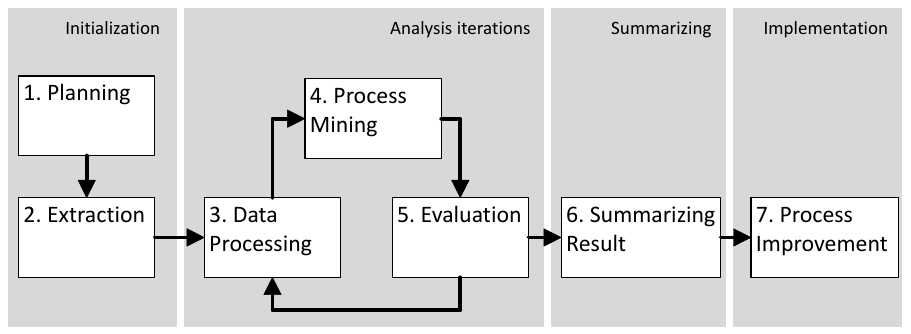
\includegraphics[width=14cm]{Chapters/Notizen_Graphics/ProcessMiningSteps.jpg}
\caption{Steps in Process Mining\protect\cite{Buijs2017}} 
\end{figure}

\noindent The DHM is a new mining method and thus the main focus lies on step 4. and only partly on 3. and 5. when reproducing the results and testing further functionalities in ProM. \protect\cite{Buijs2017}\\


\subsection{Event logs, Petri nets and model criteria}
Event logs store information about \textbf{activities} and each execution of a process produces a sequence of \textbf{events}. Events are stored with attributes $A$ and values $U$ in traces $\sigma \in \mathscr{L}$.\\
Thus an event log $L = (E, \Sigma, \#, L)$ consists of:


\begin{itemize}
\setlength{\itemsep}{3pt}
\item{$E$ - a finite set of unique event identifiers}
\item{$\Sigma \subseteq U$ - a finite set of activities}
\item{$\# : E \rightarrow (A \nrightarrow U)$ - attribute values recorded for an event}
\item{$\mathscr{L} \subseteq E\text{*}$ - the set of traces over E}
\item{$\sigma \in \mathscr{L}$ - traces, which record the sequence of events for
one process instance - each event occurs only in a single trace}
\end{itemize}

\noindent In the following figure this can be seen for three traces with attributes \textbf{act}ivity, \textbf{p}riority, \textbf{n}urse and \textbf{t}ype. The emergency ward example will be used throughout this paper and in Chapter three it will be explained in more detail, when reproducing the results for the DHM. \protect\cite{Mannhardt17}

\begin{figure}[H]
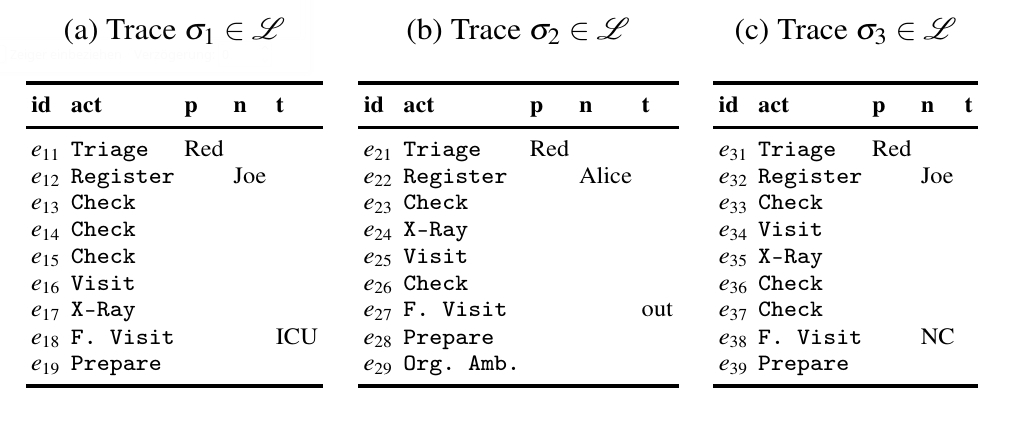
\includegraphics[width=14cm]{Chapters/Graphics_Paper/Event_Traces_ex_HB.jpg}
\caption{Three traces of an example process of the emergency ward data \protect\cite{Mannhardt17}} 
\end{figure}

\noindent While the data is presented in event logs - consisting of traces, the model derived from it, can be displayed in  graphical form (i.e. Petri net, C-net, BPMN). Common patterns, which can be displayed by a Petri net are Sequences, Choice [e, f], Parallelism [b, c, d], and Loops.

\begin{figure}[H]
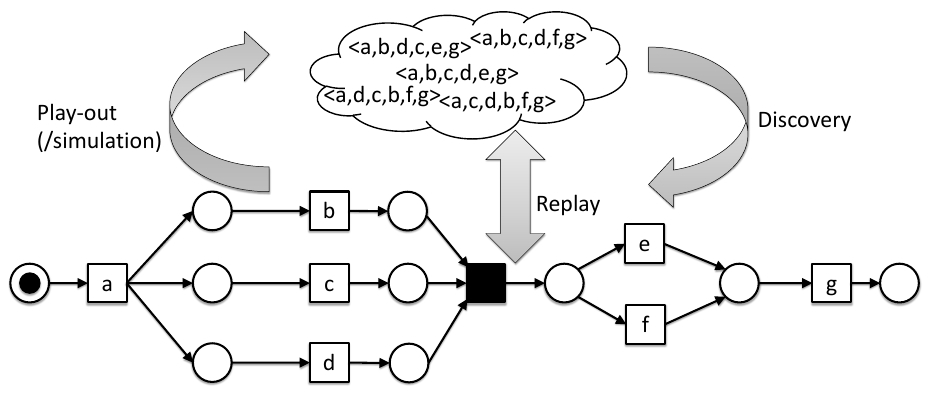
\includegraphics[width=14cm]{Chapters/Notizen_Graphics/ProcessModel_Behaviour.jpg}
\caption{A Petri net derived from Event logs\protect\cite{Buijs2017}} 
\end{figure}

\noindent Once a model has been discovered the following criteria should be considered:

\begin{enumerate}
\setlength{\itemsep}{3pt}
\item Soundness: Are the criteria for Soundness met?
\item Replay Fitness: Can all traces be represented by the model?
\item Precision: Can the model represent additional cases, not seen in the traces? 
\item Generalization: Is the model restrictive or can it be applied in general?
\item Simplicity: Is the model as simple as possible?
\end{enumerate}

\vspace{5mm}
\textbf{Soundness}
\begin{enumerate}
\setlength{\itemsep}{3pt}
\item{Option to complete}\\
For each possible state of the process model, it is possible to reach the end state

\item{Proper completion}\\
When the process model reaches the end state, there are no tokens left behind

\item{No dead transitions}\\
Each transition in the process model can be enabled\\
\protect\cite{Buijs2017}
\end{enumerate}



\subsection{Causal Nets}
Conventional model notations like Petri nets and BPMN are often not able to represent observed behavior properly and discovered process models tend to have dead- or livelocks. For this reason C-nets are preferred by the authors as representation for their DHM.\\
In a Causal-net (C-net) nodes represent activities and arcs represent causal dependencies. Each activity has a set of possible input bindings and a set of possible output bindings. For example in the following Figure the Activity "Register" has one input binding from "Triage" but two sets of output bindings \{"Check", "Visit"\}, \{"Check", "X-Ray"\}. This means that "Register" is either followed by "Check" and "Visit" or "Check" and "X-Ray".\protect\cite{Mannhardt17}\protect\cite{Aalst}

\begin{figure} [H]
    \subfigure{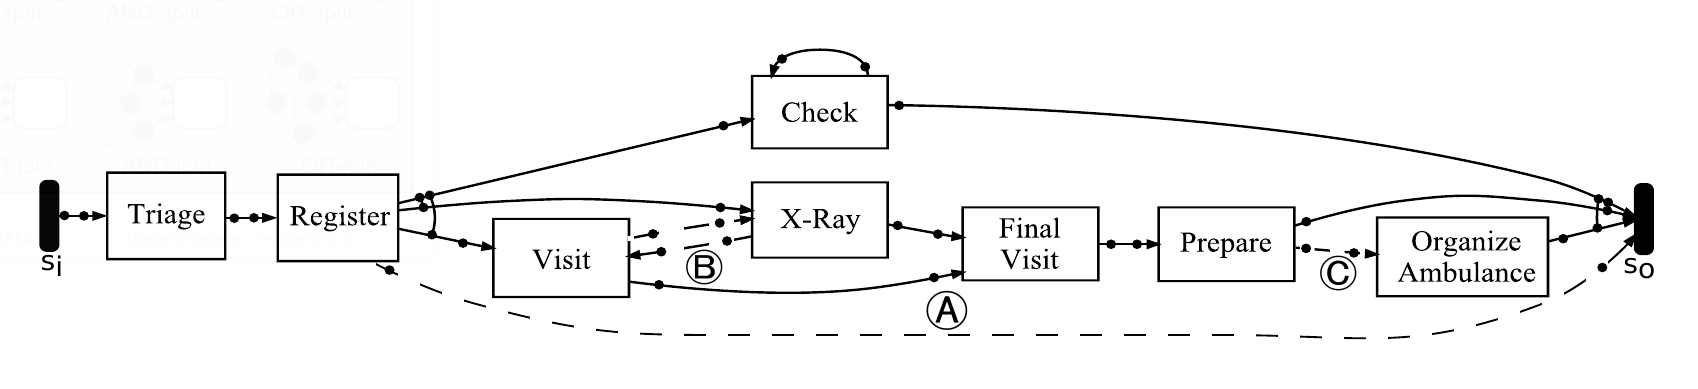
\includegraphics[width=0.7\textwidth]{Chapters/Graphics_Paper/C-net_ex_HB.jpg}}
    \subfigure{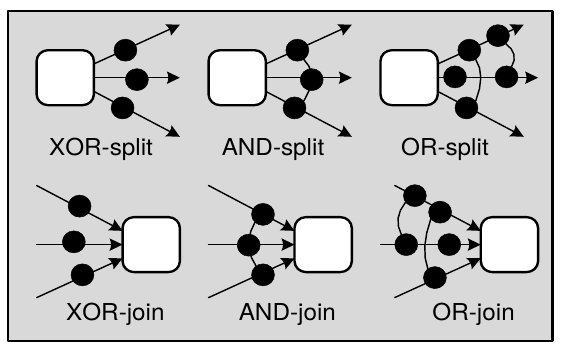
\includegraphics[width=0.25\textwidth]{Chapters/Graphics_Paper/C-nets_Legend.jpg}} 
\caption{C-net of the emergency ward example process\protect\cite{Mannhardt17}\protect\cite{VanDerAlst11}} 
\end{figure}
\vspace{3pt}

\noindent In mathematical notation a C-net is a tuple $C = (\Sigma, s_i , s_o , D, I, O)$ , consisting of:
\begin{itemize}
\setlength{\itemsep}{2pt}
\item{$\Sigma$ finite set of activities}
\item{$s_i \in \Sigma$ unique start activity}
\item{$s_o \in \Sigma$ unique end activity}
\item{$D \subseteq \Sigma \times \Sigma$ dependency relation}
\item{$B = \{X \subseteq \mathscr{P} (\Sigma) \; \rvert \; X = \{ \varnothing \} \vee \varnothing \notin X \} $ possible bindings}
\item{$I \in \Sigma \rightarrow B$ set of input bindings per activity}
\item{$O \in \Sigma \rightarrow B$ set of output bindings per activity}\\
\protect\cite{Mannhardt17}
\end{itemize}



%----------------------------------------------------------------------------------------

\section{Mining Methods}
In order to discover an adequate process model the DHM builds on methods, which are applied in several established miners. The concepts of relation notation, footprint-/ dependency matrices and classification by decision trees in an event log, will be briefly introduced in connection to the respective miner.  

\subsection{Alpha Miner}
This very basic miner was the first to bridge from Event Logs to Petri nets. First a footprint matrix is detected from the event log. By applying the following notation, it can be interpreted from the symmetric matrix, that b follows a, but e, f and g never follow a.\\

\begin{tabular}[width=13cm]{llll}
$>$ & Directly follows &a $>$ b& a is directly followed by $b$ \\
$\rightarrow$ & Sequence & a $\rightarrow$ b & if $a>b$ and not $b>a$ \\
|| & Parallel & a || b & if both a > b and b > a \\
$\#$ & No direct relation & a $\#$ b & if neither $a>b$ and $b>a$ \\
\end{tabular}


\begin{figure}[H]
\begin{center}
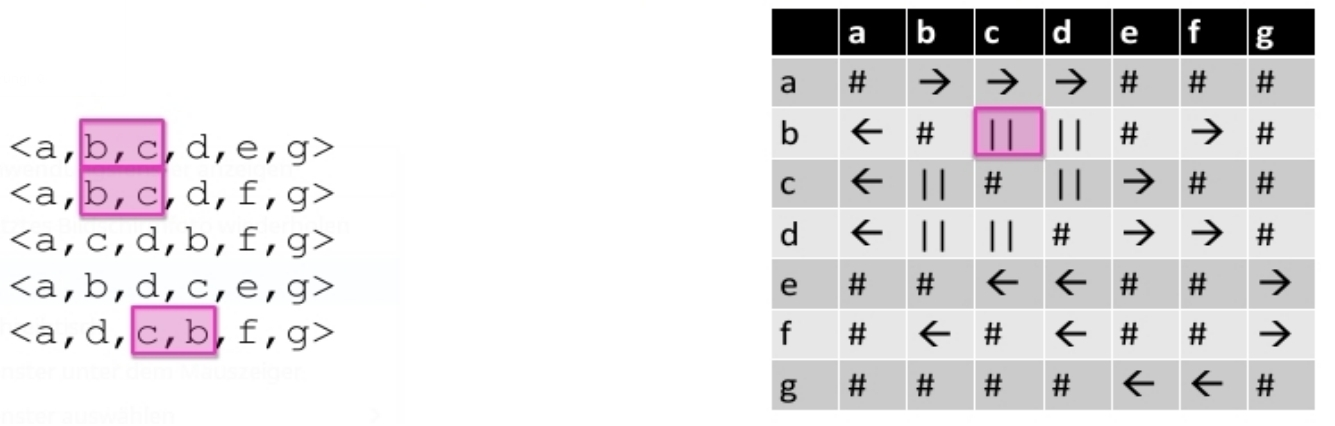
\includegraphics[width=0.8\textwidth]{Chapters/Graphics_Paper/AlphaMiner_DependenceMatrix.jpg}
\caption{The Footprint Matrix of the Alpha Miner\protect\cite{Buijs2017}} 
\end{center}
\end{figure}

\noindent From the footprint matrix the following Petri net can be derived. The actions b, c and d, which were marked as parallel in the above Figure, are now displayed as parallel paths.\protect\cite{Buijs2017}

\begin{figure}[H]
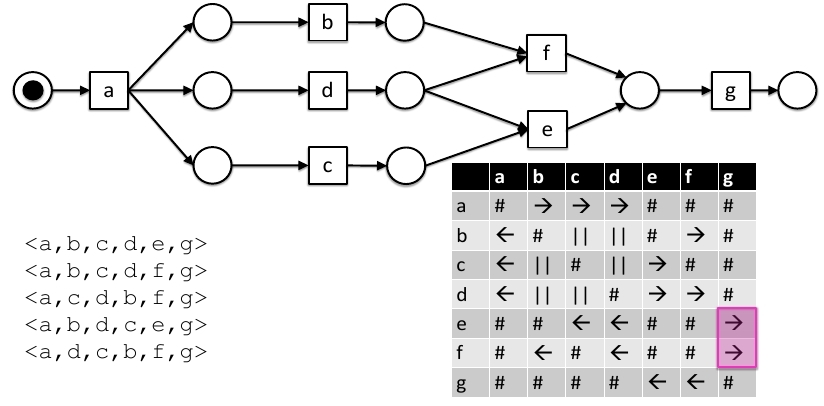
\includegraphics[width=0.9\textwidth]{Chapters/Notizen_Graphics/Notation_FootprintMatrix_PetriNet.jpg}
\caption{A derived Petri net of the Footprint Matrix\protect\cite{Buijs2017}} 
\end{figure}

\subsection{Heuristics Miner (HM)}
The Heuristic Miner is an Improvement of the Alpha miner, as it takes frequencies into account, detects short-loops and can detect skipping activities. However it does not guarantee for sound process models.\\

\noindent The basic idea is, to count the relations in the footprint matrix and calculate relative frequencies which returns a dependency matrix, as depicted in the following Figure.

\begin{figure}[H]
\begin{center}
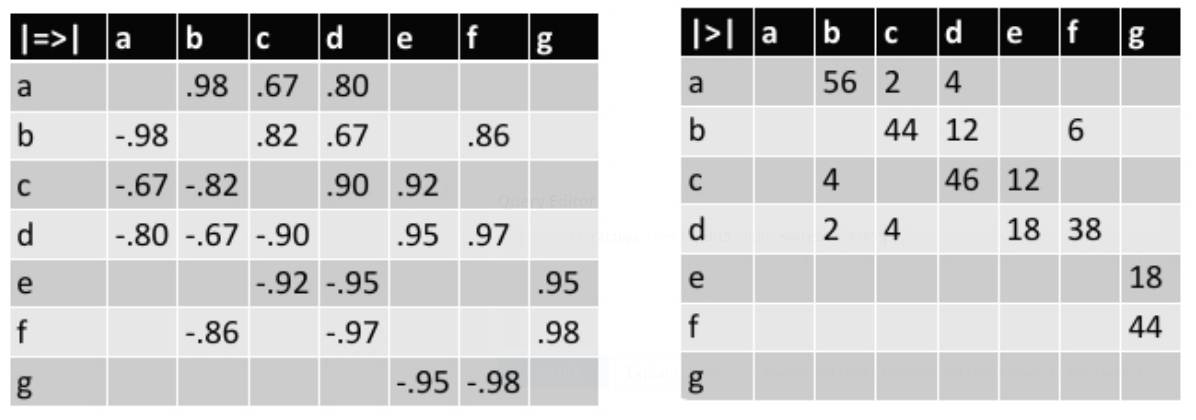
\includegraphics[width=0.7\textwidth]{Chapters/Graphics_Paper/HeuristicMiner_DependencyMatrix.jpg}
\caption{Dependency Matrix des Heuristic Miners\protect\cite{Buijs2017}} 
\end{center}
\end{figure}
\[a => b = \frac{|a>b|-|b>a|}{|a>b|-|b>a|+1}\]
\vspace{5pt}


\noindent It can be seen that the frequency of |a>b| - meaning a was followed by b - is 56. The opposite |b>a| never occurred and for this reason, by applying the formula above, the relative frequency or "significance of the dependency" of 0.98 can be calculated. The opposing relative frequency of -0.98 can be derived from the first result and is inserted in the matrix as well.\protect\cite{Buijs2017}


\subsection{Inductive Miner (IM)}
With the Inductive Miner the idea of classification by decision trees is introduced to process mining and because it doesn't use Petri nets, it guarantees sound process models.
The IM repeatedly finds the most prominent splits in the event log, then detects the operator (e.g. X) and afterwards continues on both sublogs.\\
In the following Figure the example event log from this chapter is first split into the most prominent activities a (start) and g (end). Afterwards the OR operator is applied for e and f and finally b,c and d are split with and the parallel operator detected for this split.\protect\cite{Buijs2017}

\begin{figure} [H]
    \subfigure[Always a]{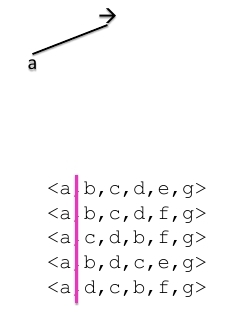
\includegraphics[width=0.34\textwidth]{Chapters/Notizen_Graphics/InductMin_repeat1.jpg}} 
    \subfigure[Always e OR f]{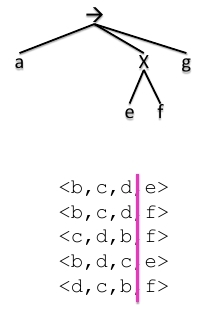
\includegraphics[width=0.3\textwidth]{Chapters/Notizen_Graphics/InductMin_repeat2.jpg}}
    \subfigure[Parallelism b,c,d]{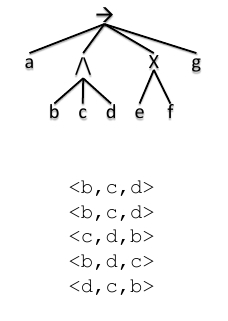
\includegraphics[width=0.33\textwidth]{Chapters/Notizen_Graphics/InductMin_repeat3.jpg}} 
\caption{Inductive Miner - Repeatedly Split Event Log\protect\cite{Buijs2017}} 
\end{figure} 


%----------------------------------------------------------------------------------------
\section{The Data-aware Heuristic Miner (DHM)}
\subsection{Data-aware Dependency Measures}
In contrast to the miners which have been shortly presented in this chapter, the DHM is supposed to also consider and evaluate infrequent but data-dependent process behavior. Rare events are either vastly disregarded as noise e.g. by the HM or not properly filtered e.g. by the IM.
\begin{figure} [H]
    \subfigure[Inductive Miner]{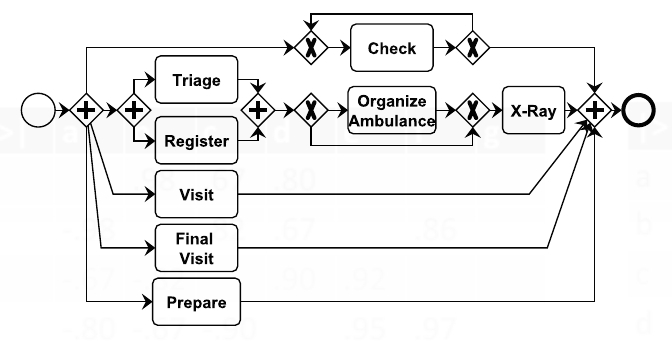
\includegraphics[width=0.49\textwidth]{Chapters/Graphics_Paper/IM_ex_HB.jpg}}
    \subfigure[Heuristic Miner]{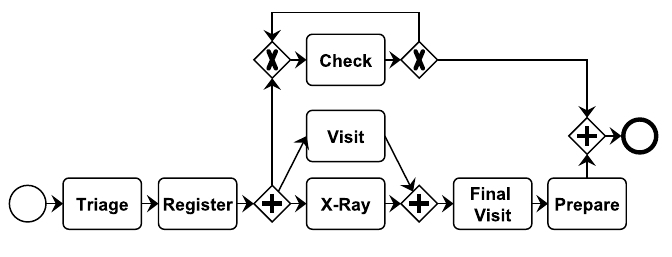
\includegraphics[width=0.49\textwidth]{Chapters/Graphics_Paper/HM_ex_HB.jpg}} 
\caption{Discovered models by the IM and HM in BPMN \protect\cite{Mannhardt17}}
\end{figure}

\noindent The approach of Mannhardt et. al is to extend the HM with a measure for conditional dependency. Binary classifiers are applied to predict directly-follows relations based on attribute values recorded in the event log.\\ 
\noindent Those classifiers are denoted as \textbf{Dependency Conditions}:
\[C_a,_b(x) = (C(a, b))(x)\]
This binary classifier predicts whether an event of activity a is directly followed by an event of activity b for the attribute values x. This means that $C_a,_b(x) = 1$ when b is predicted to directly follow a and $C_a,_b(x) = 0$ when a different activity is predicted.\\


\noindent Given $a, b \in \Sigma$ and dependency conditions C, the frequency with which b is observed to directly follow a is derived from the event log. This relation is denoted as:
\noindent\textbf{Conditional directly follows relation}
\[a >^{C,L} b\]
An execution of activity a with the latest attribute values x is directly followed by an execution of activity b under dependency condition $C_a,_b(x)$.

\noindent The \textbf{Conditional dependency measure} is calculated analogous to the dependency measure described for the HM earlier. The authors define 
$a => ^{C,L}b: \Sigma \times \Sigma \rightarrow [-1, 1]$ as the strength of the causal
dependency from a to b under condition $C_{a,b}$ in the event log:

\[a => ^{C,L}b = 
\begin{cases}
		\frac{|a>^{C,L}b|-|b>^{C,L}a|}{|a>^{C,L}b|-|b>^{C,L}a|+1} & \text{for a} \neq b,\\
		\frac{|a>^{C,L}b|}{|a>^{C,L}b|+1} & \text{otherwise}.
\end{cases}
\]

\noindent The difference to the earlier measure is the data-aware dependency condition. 
If a relation (a, b) is clearly characterized by a certain dependency condition $C_{a,b}$ it should be included in the dependency relations of the discovered causal net.\\

\noindent The \textbf{emergency ward example} will provide a better understanding of the described measures. An event log L with 50 traces for each of the three $\sigma_{1-3}$ was introduced earlier and will be used in the following steps:
\begin{enumerate}\setlength{\itemsep}{1pt}
\item Determine the conditional dependency measure $X => ^{C,L} V$ from activity X-Ray (X) to activity Visit (V)\\
=> Assumtion that condition $C_{X,V}(v) = 1$ only if attribute Nurse = Alice
\item Obtain the number of times X is directly followed by V under condition $C_{X,V}$\\
=> $|X >^{C,L} V|$ = 50
\item Obtain the number of times V is directly followed by X under conditions C \\
=> $|V >^{C,L} X|$ = 0
\item Derive the conditional dependency measure under C \\
=> $X => ^{C,L} V = \frac{50-0}{50+0+1} \approx 0.98$
\end{enumerate}
This indicates a strong dependency relation from activity X to activity V under condition $C_{X,V}$ . By contrast, if we consider the unconditional dependency measure $X => ^{1,L} V$, then we obtain $\frac{50-100}{50+100+1} \approx -0.33$.
Thus, when disregarding the data perspective, both activities appear to be executed in parallel.\protect\cite{Mannhardt17}

\subsection{Training a classifier for the dependency condition}
The \textbf{dependency condition} which was introduced above, is the basis of the other two definitions and thus the first step when applying the DHM in order to decide which relations should be included in the C-net.\\
A set of training instances is built for every combination of activities $(a, b) \in \Sigma \times \Sigma$.

\noindent \textbf{Training Instances} are defined by:
\begin{itemize}
\item $ a \in \Sigma$ the given source activity
\item $ b \in \Sigma$ the candidate activity
\item $ \theta_{dep} \in [0,1]$ the dependency threshold
\end{itemize}

\noindent Then $ a\bullet \subseteq \Sigma$ is the set of activities s that directly follow a in the event log with an unconditional dependency measure above the threshold $ \theta_{dep} $ , i.e., 
\[a\bullet = {s \in \Sigma | a => ^{1,L} s \geq \theta_{dep}}\]

\noindent We collect those events $X_{L,a,b} \subseteq E$ that directly follow an execution of a in the event log, and refer to activities in $a\bullet$, or to the candidate activity b, i.e.,  \[X_{L,a,b} = {e \in E | \bullet(e) = a \wedge \#_{act} (e) \in a\bullet \cup \{b\}}\]

\noindent Function $T_{L,\theta_{dep}}\in (\Sigma \times \Sigma) \rightarrow B((A \nrightarrow U) \times {1, 0})$ returns the multi-set of training instances:
\[T_{L,\theta_{dep}} (a, b) = \biguplus _{e \in X_{L,a,b}} [(val(e), cl(e))] with cl(e) =
\begin{cases}
1, & for \#_{act}(e)=b,\\
0, & for \#_{act}(e)\neq b
\end{cases}
\]

\noindent This method is conceptually independent of the used classification algorithm. The authors employed \textbf{decision trees (C4.5)} as they are efficient and provide results in human interpretable conditions.\\
To build the \textbf{dependency conditions C}:
\begin{enumerate}
\item A set of training instances $T_{L,\theta_{dep}} (a, b)$ is assembled.
\item A decision tree for each possible relation $(a, b) \in \Sigma \times \Sigma$ is trained.
\item A score $q(C_{a,b}) \in [0, 1]$ is used to determine the quality of a condition $C_{a,b}$.
\end{enumerate}

\noindent As a performance measure the authors opted for Cohen’s kappa ($\kappa$), which indicates whether the prediction was better than a prediction by chance (i.e., for $\kappa$ > 0).\\

\noindent Again the \textbf{emergency ward example} with an event log of 150 traces will provide a better understanding of the just described methods.\\
\noindent The dependency threshold shall be $\theta_{dep} = 0.9$ and the classifier for the dependency condition $C_{X,V}$, i.e., the dependency relation from X-Ray (X) to Visit (V) will be trained:

\begin{enumerate}
\item The training instances are $T_{L,\theta_{dep}}(X,V ) = [(v1, Final Visit)^{50} , (v2, Visit)^{50} ]$
\item The attribute value functions are $v1 (P) = Red$, $v1 (N) = Joe$ and $v2(P) = Red$, $v2 (N) = Alice$ 
\item A C4.5 decision tree is trained and the dependency condition $C_{X,V}$ with $C_{X,V} (v2 ) = 1$ and $C_{X,V} (v1) = 0$ is obtained
\end{enumerate}

\noindent There is no instance with the activity Check (C) since the unconditional dependency measure $X => ^{1,L}C$ is below the threshold of 0.9. So the instances based on trace $\sigma 3$ are not included because activity C is in parallel to X.\protect\cite{Mannhardt17} 

\subsection{Tuning noise filtering capabilities and discovering C-nets}
In order to filter the noise from rare events the DHM supports four user-specified thresholds which range between 0 and 1:
\begin{itemize}
\item $\theta_{obs}$, observation threshold - controlling the relative frequency of relations
\item $\theta_{dep}$, dependency threshold - controlling the strength of causal dependencies
\item $\theta_{bin}$, binding threshold - controlling the number of bindings
\item $\theta_{con}$, condition threshold - controlling the quality of data dependencies
\end{itemize}

\noindent A C-net tuple $C = (\Sigma, s_i , s_o , D, I, O)$ is derived from an event log $L = (E, \Sigma, \#, L)$ and the thresholds $\theta_{obs}$, $\theta_{dep}$, $\theta_{bin}$, $\theta_{con}$, in the following steps.

\begin{enumerate}
\item Add artificial start and end events to all traces to ensure unique start and end activities $s_i$ and $s_0$
\item Build the set of standard dependency relations
\item Discover the dependency conditions C by training the classifiers for each pair (a, b), using the training instances $T_{L,\theta_{dep}} (a, b)$.
\item Add the conditional dependency relations C to D, using $\theta_{con}$ instead of $\theta_{obs}$ to
obtain infrequent, high-quality data conditions
\item Handle activities $s \in \Sigma$ which don't have a predecessor or successor in the directed
graph induced by D. As all tasks in the C-net should be connected, two alternative heuristics are proposed by the authors: \textbf{all-task-connected} and \textbf{accepted-task-connected}. The latter one connects repeatedly only those activities that are already part of the dependency graph using their best neighboring activities until all activities have a cause and an effect.\\
$\bar{D}$ denotes the set of relations necessary to connect all activities accepted so far. Afterwards the dependency relations with the new relations, i.e., $D = D \cup \bar{D}$ is extended. As now there might be new, unconnected activities in $\bar{D}$ the steps are repeated i.e. the best neighboring activities are added until set $\bar{D}$ is empty.
\item The input and output binding functions of the C-net are discovered. We discover the input ($I$) and output ($O$) binding functions of the C-net. To find $O(a)$ it has to be determined which of the executions of b were caused by an execution of activity a. Using the same heuristic like before activity a only is considered to have caused b if it is the nearest activity. Any other activity s executed in between a and b should not be a possible cause of b. $\bar{O}$ denotes the set of activities that were caused by event $e_i$.

The frequency $|o|_{L,a} \in N$ of an output binding $o \subseteq \Sigma$ for activity $a \in \Sigma$
in the event log L is determined as:
\[O(a) = \{{o \subseteq \Sigma | \frac{|o|_{L,a}}{max_{\bar{o}\subseteq \Sigma}(|\bar{o}|_{L,a})}\geq \theta_{bin}}\}\]\\
The input binding function $I$ is obtained by reversing the same approach.\protect\cite{Mannhardt17}
\end{enumerate}


























 
% Chapter3

\chapter{Result Reproduction} % Main chapter title

\label{Chapter3} % For referencing the chapter elsewhere, use \ref{Chapter1} 

%----------------------------------------------------------------------------------------

% Define some commands to keep the formatting separated from the content 
%\newcommand{\keyword}[1]{\textbf{#1}}
%\newcommand{\tabhead}[1]{\textbf{#1}}
%\newcommand{\code}[1]{\texttt{#1}}
%\newcommand{\file}[1]{\texttt{\bfseries#1}}
%\newcommand{\option}[1]{\texttt{\itshape#1}}


%----------------------------------------------------------------------------------------


\section{Synthetic Data Logs}

\subsection{Evaluation design and methods}
The authors generated an event log with 100,000 traces and approximately 900,000 events.\\

\begin{table}[H]
\begin{tabularx}{\textwidth}
{>{\setlength\hsize{0.8\hsize}\setlength\linewidth{\hsize}}
X>{\setlength\hsize{1.2\hsize}\setlength\linewidth{\hsize}}
X>{\setlength\hsize{1\hsize}\setlength\linewidth{\hsize}}
X}
\textbf{Attributes} & \textbf{Methods} & \textbf{Thresholds} \\
\hline
\noindent
\begin{itemize}[leftmargin=*] 
\item Priority (P) \newline white 1.4\%
\item Nurse (N) \newline Alice 19.1\%
\item Type (T) \newline out 4.3\%
\end{itemize} &
\begin{itemize}[leftmargin=*] 
\item DHM
\item HM - frequency filter (HMF)
\item HM - no frequency filter (HMA)
\end{itemize} &
\begin{itemize}[leftmargin=*] 
\item $\theta_{obs}$ = 0.06 \newline (0.0 for HMA)
\item $\theta_{dep}$ = 0.9
\item $\theta_{bin}$ = 0.1
\item $\theta_{con}$ = 0.5
\end{itemize}
\end{tabularx}
\end{table}

\noindent
Furthermore the \textbf{accepted-task-connected heuristic} was used, the \textbf{C4.5} applied as the classifier and its performance was estimated using \textbf{10 times 10-fold cross validation}.

%----------------------------------------------------------------------------------------

\section{Hospital Billing}
The Hospi-
tal Billing (HB) event log was obtained from the ERP system of a hospital. It contains
100,000 cases with 550,000 events and 38 data attributes related to the billing of medical
services.

CaseType
CloseCode
isClosed
Speciality

%----------------------------------------------------------------------------------------

\section{Road Fines}
The Road Fines (RF) event log was recorded by an information system that handles road-traffic fines by an Italian local police force. This event log contains about 150,000 cases, 500,000 events, and 9 data attributes. 

We applied the proposed method (DHM), the HM with the same frequency fil-
ter settings (HMF) and the Inductive Miner (IM) to both event logs. 
Without a reference
model and knowledge about expected noise levels, we could not compare the discov-
ered models to a gold standard. Therefore, we compare the novel insights obtained by
using our method with those from the other methods.


  
%% Notizen

\chapter{Notizen} % Main chapter title

\label{Notizen} % For referencing the chapter elsewhere, use \ref{Chapter1} 

%----------------------------------------------------------------------------------------

% Define some commands to keep the formatting separated from the content 
%\newcommand{\keyword}[1]{\textbf{#1}}
%\newcommand{\tabhead}[1]{\textbf{#1}}
%\newcommand{\code}[1]{\texttt{#1}}
%\newcommand{\file}[1]{\texttt{\bfseries#1}}
%\newcommand{\option}[1]{\texttt{\itshape#1}}


%----------------------------------------------------------------------------------------

\section{C-Nets}

Causal nets (C-nets) -> a tuple $(\Sigma, s_i , s_o , D, I, O)$\\

\begin{itemize}
\item{$\Sigma$ endliches Set an Aktivitäten}
\item{$s_i \in \Sigma$ eindeutige Start Aktivität}
\item{$s_o \in \Sigma$ eindeutige Ende Aktivität}
\item{$D \subseteq \Sigma \times \Sigma$ Abhängigkeitsbeziehung}
\item{$B = \{X \subseteq \mathscr{P} (\Sigma) \; \rvert \; X = \{ \varnothing \} \vee \varnothing \notin X \} $  mögliche Bindunge}
\item{$I \in \Sigma \rightarrow B$ Set der Input Bindungen pro Aktivität}
\item{$O \in \Sigma \rightarrow B$ Set der Output Bindungen pro Aktivität}

\end{itemize}
%--------------------------------------------------------------------------------------


\pagebreak
\section{ProM Schulung}

\begin{figure}[H]
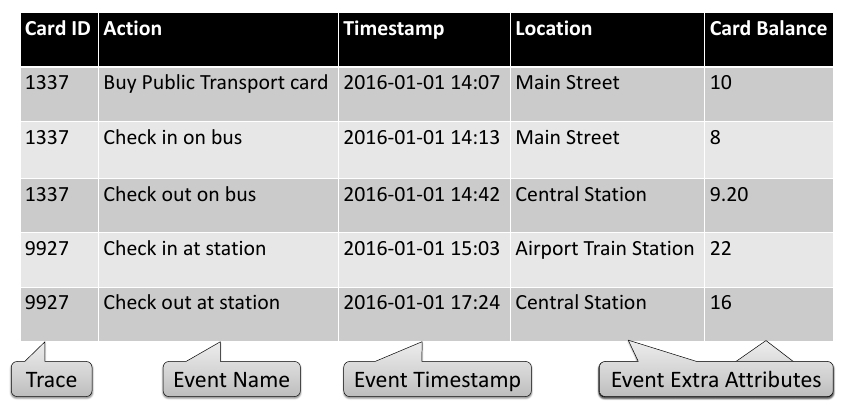
\includegraphics[width=14cm]{Chapters/Notizen_Graphics/TransportEventData.jpg}
\caption{Eventdaten eines Transportprozesses} 
\end{figure}

\begin{figure}[H]
\vspace*{.04\textheight}
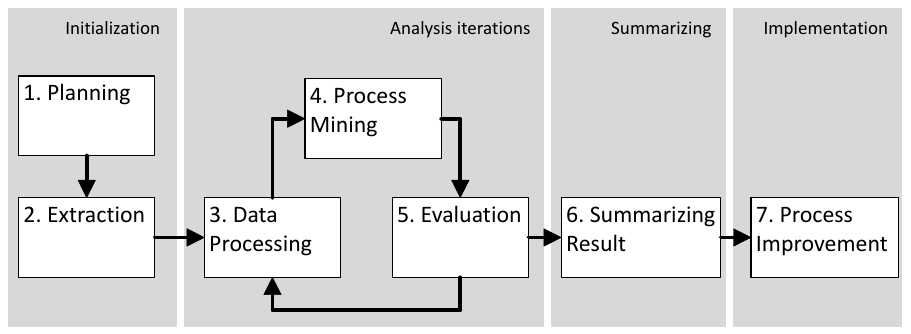
\includegraphics[width=14cm]{Chapters/Notizen_Graphics/ProcessMiningSteps.jpg}
\caption{Schritte des Process Mining} 
\end{figure}

\subsection{Petrinets}

\textbf{Petrinet Notation}
\begin{figure}[H]

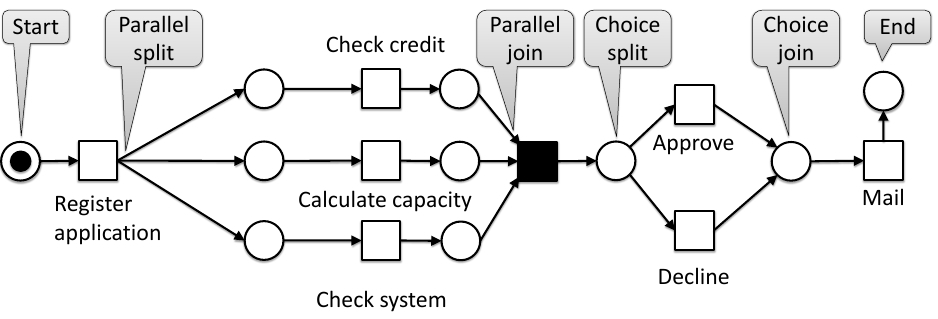
\includegraphics[width=14cm]{Chapters/Notizen_Graphics/Petri_Notation.jpg}
\caption{Petrinets Notation} 
\end{figure}

\begin{figure}[H]
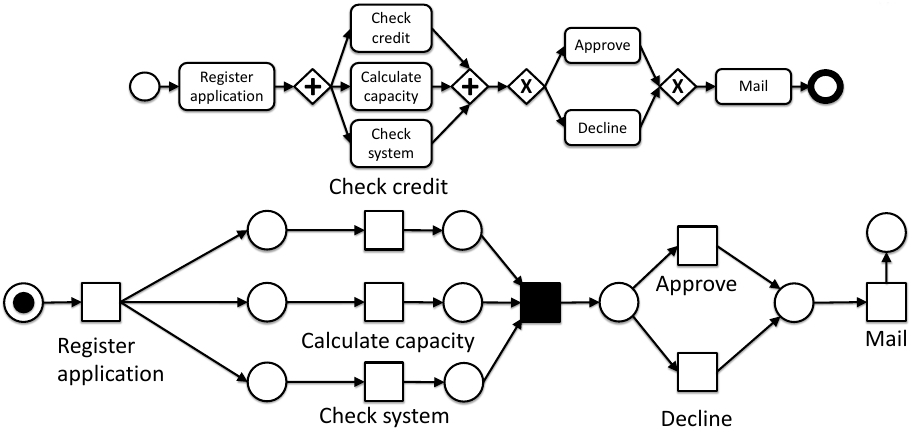
\includegraphics[width=14cm]{Chapters/Notizen_Graphics/Petri_BPMN_Notation.jpg}
\caption{Petrinets Notation vgl. mit BPMN} 
\end{figure}


\subsection{Recognize Patterns}
The goal is to discover a process model from event logs.
After the discovery follow conformance and enhancement as process mining procedures.

\begin{figure}[H]
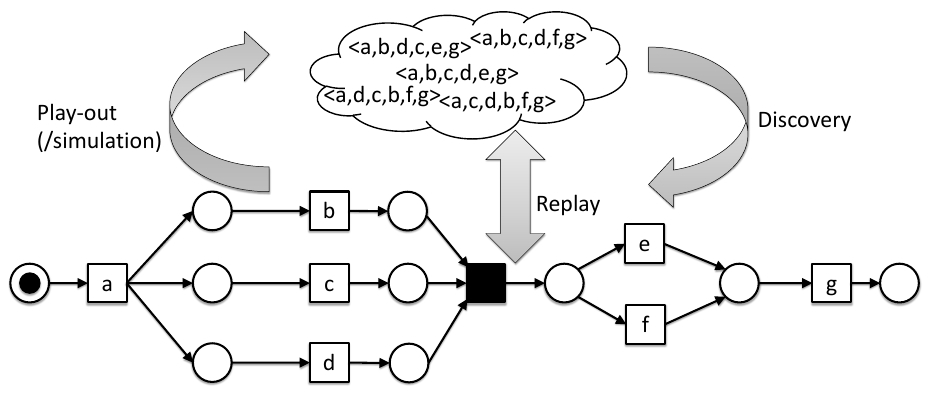
\includegraphics[width=14cm]{Chapters/Notizen_Graphics/ProcessModel_Behaviour.jpg}
\caption{Ableitung des Petrinets aus Eventlogs} 
\end{figure}

Common patterns:
\begin{itemize}
\setlength{\itemsep}{0.4mm}
\item{Sequence}
\item{Choice}
\item{Parallelism}
\item{Loops}
\end{itemize}

\begin{figure}[H]
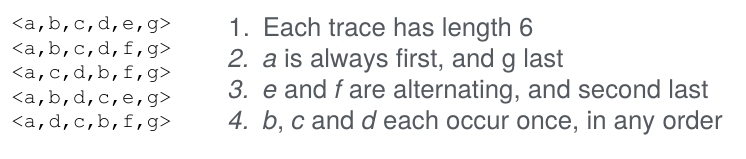
\includegraphics[width=14cm]{Chapters/Notizen_Graphics/Recognize_Patterns.jpg}
\caption{Muster in Traces erkennen} 
\end{figure}

\textbf{Detect and ignore noise}
\begin{figure}[H]
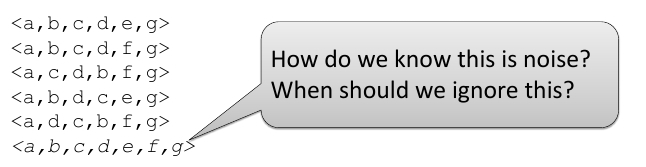
\includegraphics[width=14cm]{Chapters/Notizen_Graphics/Detect_Noise.jpg}
\caption{Hintergrundrauschen/ Noise erkennen} 
\end{figure}

\vspace{5mm}\pagebreak
\textbf{Main challenges in process discovery}
\begin{enumerate}
\setlength{\itemsep}{3pt}
\item{Discover sound process models}
\item{Recognize patterns}
\item{Detect and ignore noise}
\item{Generalize from observations}
\end{enumerate}

\vspace{5mm}
\textbf{Process model checklist}
\begin{enumerate}
\setlength{\itemsep}{3pt}
\item Soundness: Are the criterion for Soundness met?
\item Replay Fitness: Can all traces be represented by the model?
\item Precision: Can the model represent additional cases, not seen in the traces? 
\item Generalization: Is the model restrictive or can it be applied in general?
\item Simplicity: Is the model as simple as possible?
\end{enumerate}

\vspace{5mm}
\textbf{Soundness}
\begin{enumerate}
\setlength{\itemsep}{3pt}
\item{Option to complete}\\
For each possible state of the process model, it is possible to reach the end state

\item{Proper completion}\\
When the process model reaches the end state, there are no tokens left behind

\item{No dead transitions}\\
Each transition in the process model can be enabled
\end{enumerate}

\pagebreak
\section{Different Miners}
\subsection{Alpha Miner}
Very first Miner to bridge from Event Logs to Petri Nets - Mining Process Models.

\begin{enumerate}
\item Detects Footprint Matrix
\item Derives PetriNet
\end{enumerate}

\begin{figure}[H]
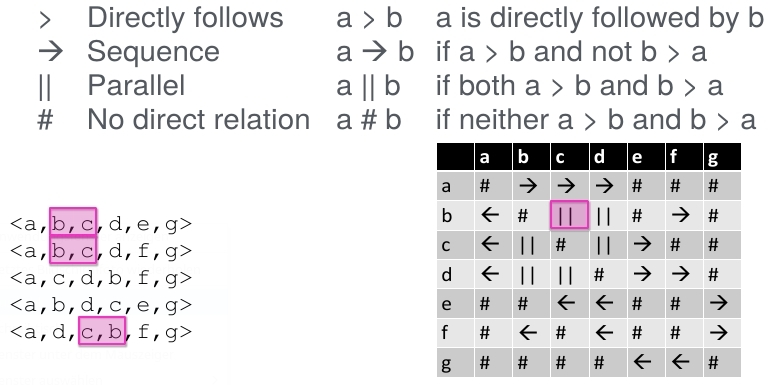
\includegraphics[width=14cm]{Chapters/Notizen_Graphics/Notation_FootprintMatrix.jpg}
\caption{Notation and the Footprint Matrix} 
\end{figure}

\begin{figure}[H]
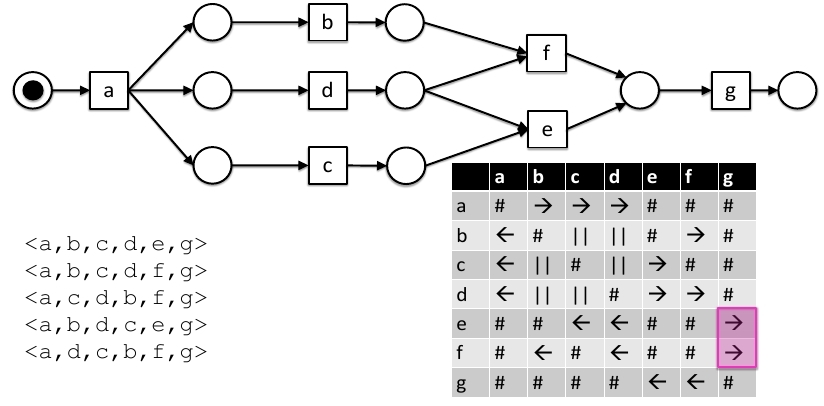
\includegraphics[width=14cm]{Chapters/Notizen_Graphics/Notation_FootprintMatrix_PetriNet.jpg}
\caption{Notation and the Footprint Matrix} 
\end{figure}

\begin{figure}[H]
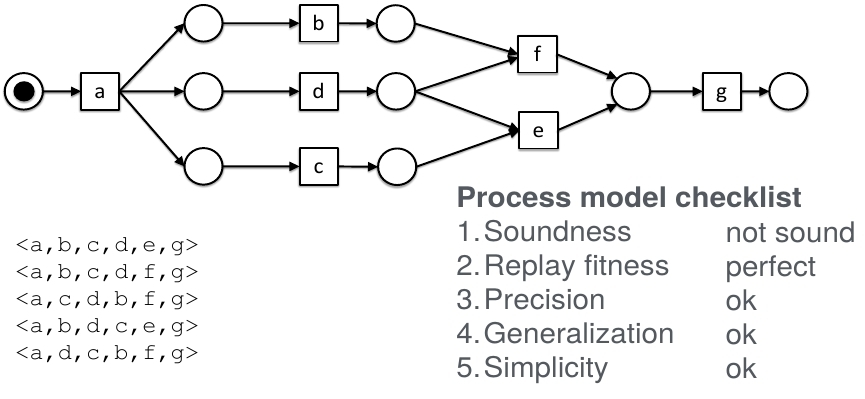
\includegraphics[width=14cm]{Chapters/Notizen_Graphics/Checklist_AlphaMiner.jpg}
\caption{Notation and the Footprint Matrix} 
\end{figure}

\section{Heuristics Miner}
\begin{itemize}
\item{Improvement of the Alpha miner}
	\begin{itemize}
	\item Takes frequencies into account
	\item Detects short-loops
	\item Detects skipping activities
	\end{itemize}
\item Does not guarantee sound process models
\end{itemize}

\begin{framed} \begin{equation}
=> = \frac{|a>b|-|b>a|}{|a>b|-|b>a|+1}
\end{equation} 
\end{framed}

\begin{figure}[H]
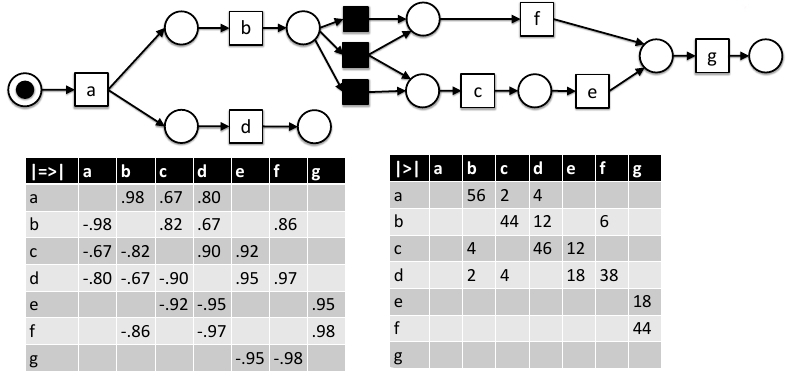
\includegraphics[width=14cm]{Chapters/Notizen_Graphics/HeuristicsMiner_Dependency_Matrix.jpg}
\caption{Dependency Matrix des Heuristic Miners} 
\end{figure}



Aus der "Frequency" rechts wird die "Significance" links berechnet. |a>b| ist die Häufigkeit in der b auf a gefolgt ist (hier 56).
-> Durch die Dependency Matrix können signifikante Abhängigkeiten erkannt werden

\begin{figure}[H]
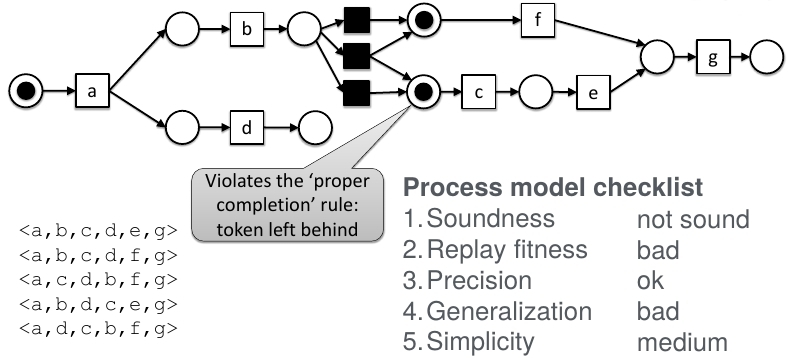
\includegraphics[width=14cm]{Chapters/Notizen_Graphics/HeuristicsMiner_conclus.jpg}
\caption{Heuristic Miner - Modell Check} 
\end{figure}


\section{Inductive Miner}
\begin{itemize}
\setlength{\itemsep}{3pt}
\item Guarantees sound process models
\item Repeatedly
	\begin{itemize}
	\item Find most prominent split in event log
	\item Detect operator
	\item Continue on both sublogs
	\end{itemize}
\end{itemize}

\begin{figure} [H]
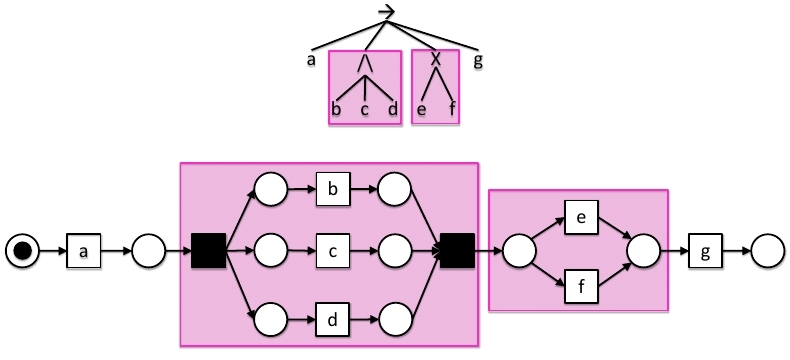
\includegraphics[width=14cm]{Chapters/Notizen_Graphics/InductMin_soundness.jpg}
\vspace*{.02\textheight}
\caption{Inductive Miner - Ableiten eines Entscheidungsbaums} 
\end{figure} 

\begin{figure} [H]
    \subfigure[Always a]{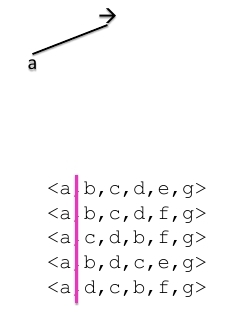
\includegraphics[width=0.34\textwidth]{Chapters/Notizen_Graphics/InductMin_repeat1.jpg}} 
    \subfigure[Always e OR f]{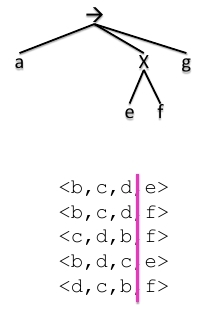
\includegraphics[width=0.3\textwidth]{Chapters/Notizen_Graphics/InductMin_repeat2.jpg}}
    \subfigure[Parallelism b,c,d]{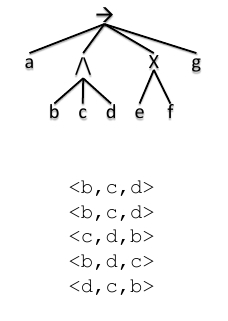
\includegraphics[width=0.33\textwidth]{Chapters/Notizen_Graphics/InductMin_repeat3.jpg}} 
\caption{Inductive Miner - Repeatedly Split Event Log} 
\end{figure} 


\begin{figure} [H]
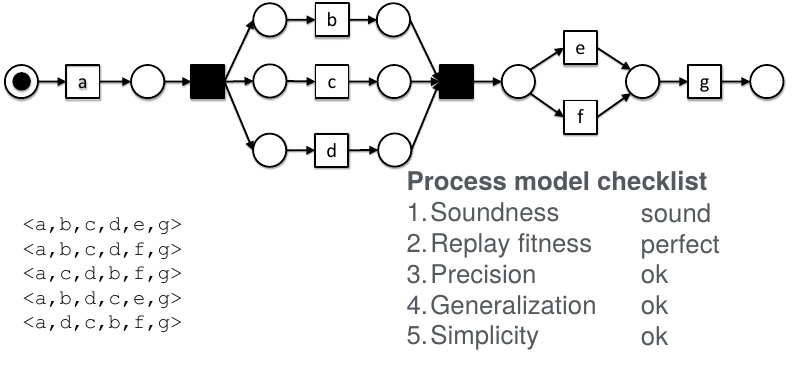
\includegraphics[width=14cm]{Chapters/Notizen_Graphics/InductMin_conclus.jpg}
\vspace*{.02\textheight}
\caption{Inductive Miner - Modell Check} 
\end{figure} 

Trennung der Traces leitet Baumstruktur und somit Modell ab.

\pagebreak
\section{Conformance Checking}
\subsection{Alignments}

Move along the trace and follow the token in the PetriNet.

\noindent\textbf{"Move on log only"}: If the arrow moved only in the trace and not in the model (i.e. f follows e in trace but not the PetriNet) the Symbol ">>" is marked down in the Model row of the Table.\\

\begin{figure} [H]
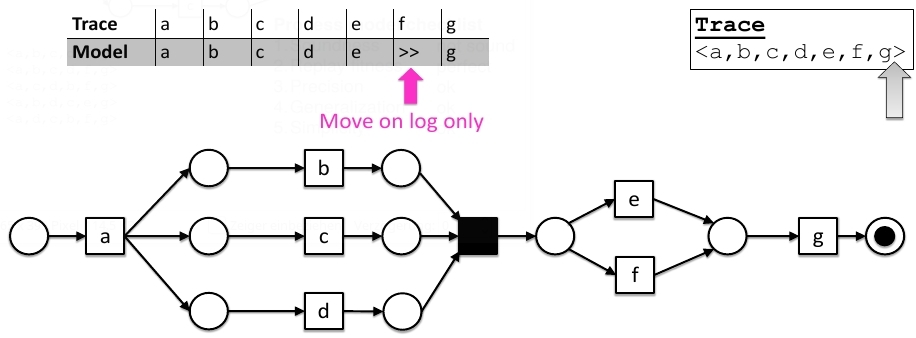
\includegraphics[width=14cm]{Chapters/Notizen_Graphics/MoveLogOnly_ConformanceCheck.jpg}
\vspace*{.02\textheight}
\caption{Compare Trace and Model} 
\end{figure} 

\textbf{This Method:}
\begin{itemize}
\item Explores multiple options to find the optimal alignment (guaranteed)
\item Allows flexible costs to activities and move types (e.g. a model move on e can be preferred over a log move on f)
\item Relates the event log to the process model and hence enables further analysis



\end{itemize}



\begin{figure} [H]
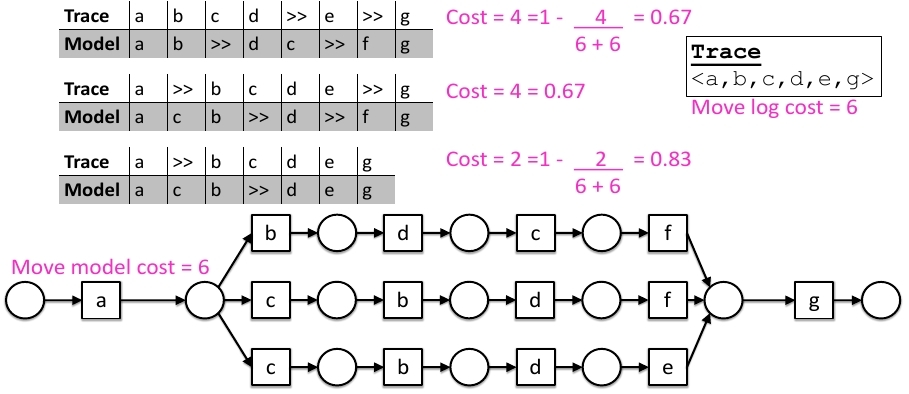
\includegraphics[width=14cm]{Chapters/Notizen_Graphics/ReplayFitness_ConformanceChecking.jpg}
\caption{Calculate Replay Fitness for each Trace} 
\end{figure} 

\begin{framed} \begin{equation}
Replay Fitness = 1 - \frac{Cost Of Allignment}{Move Log Cost + Move Model Cost}
\end{equation} 
\end{framed}


\subsection{Performance Analysis}

Normally only the \textbf{completion time} of an activity is known.\\
If the \textbf{starting time} is given as well, it is possible to distinguish between waiting and execution time. Otherwise it is only possible to calculate the time spent in one place.
\begin{figure} [H]
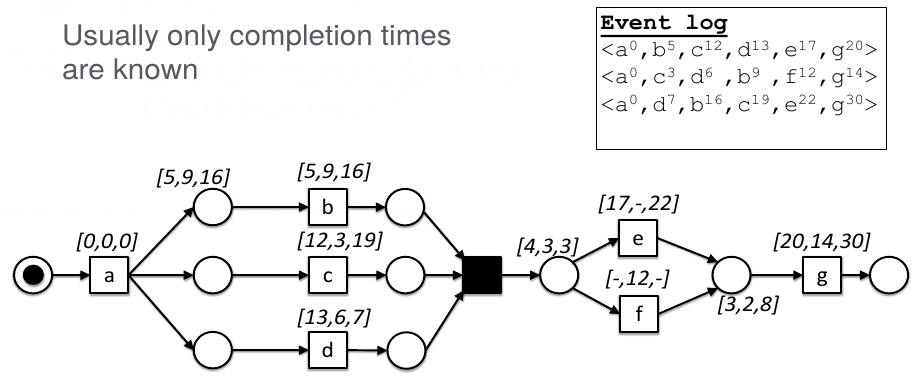
\includegraphics[width=14cm]{Chapters/Notizen_Graphics/TimestampsInTraces_PerformanceChecks.jpg}
\caption{Adding Timestamps in Traces and Modell} 
\end{figure} 


\textbf{Steps in ProM:}
\begin{itemize}
\item Load Data (here: \glqq Artificial - Loan Process.xes.gz\grqq)
\item Mine Process Model (here \glqq Mine Petri net with Inductive Miner\grqq)
\item \glqq Replay a Log on Petri nets for Performance/Conformance Analysis\grqq

\end{itemize}


\begin{figure} [H]
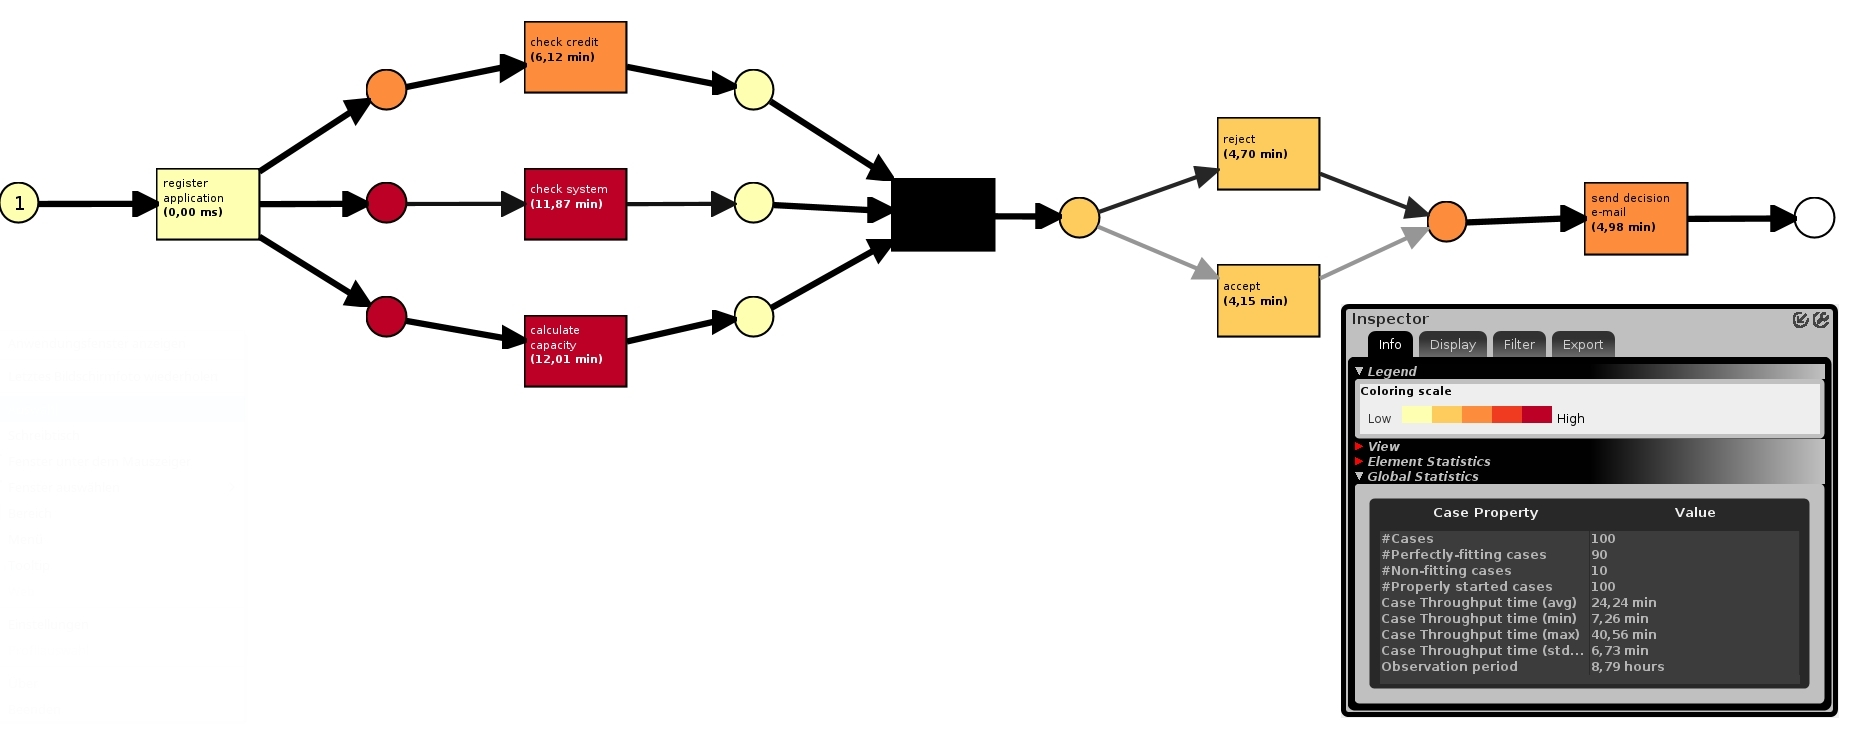
\includegraphics[width=14cm]{Chapters/Notizen_Graphics/ProM_PerformanceChecking.jpg}
\caption{Performance Checking in ProM} 
\end{figure} 

\noindent The darker red means, that the case took longer than others.\\
Question where time is spent - mainly in the parallel process, because two of them take some time and others have to wait (not sequential).\\

From the time it takes to go through certain parts of the model it might be possible to get results concerning the Conformance by analyzing deviations. (i.e. if time to complete one case is longer than average run time - possible that case is not included in every trace)


\begin{figure} [H]
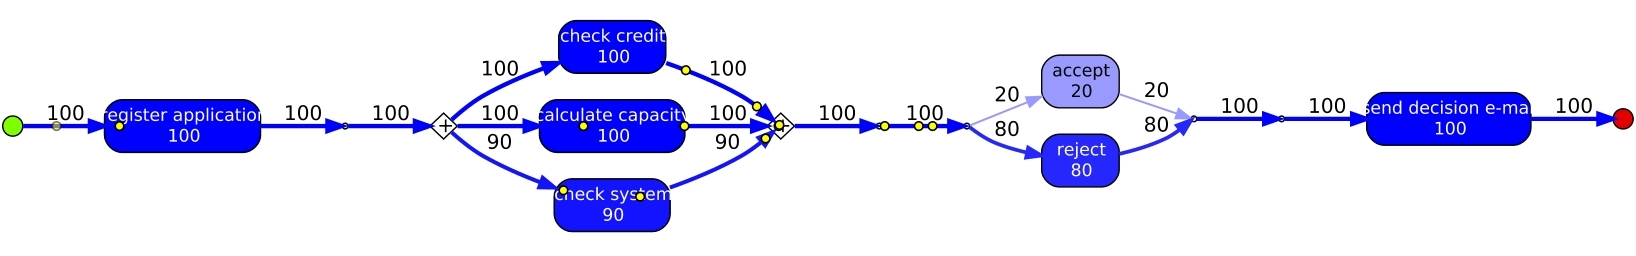
\includegraphics[width=14cm]{Chapters/Notizen_Graphics/InductiveVisualMiner_PerformanceAnalysis.jpg}
\caption{Performance Checking in ProM with the Inductive Visual Miner} 
\end{figure} 
Each transition can be seen in the graph - further 
 
%\include{Chapters/Chapter4} 
%\include{Chapters/Chapter5} 

%----------------------------------------------------------------------------------------
%	THESIS CONTENT - APPENDICES
%----------------------------------------------------------------------------------------

\appendix % Cue to tell LaTeX that the following "chapters" are Appendices

% Include the appendices of the thesis as separate files from the Appendices folder
% Uncomment the lines as you write the Appendices

%% Appendix A

\chapter{Frequently Asked Questions} % Main appendix title

\label{AppendixA} % For referencing this appendix elsewhere, use \ref{AppendixA}

\section{How do I change the colors of links?}

The color of links can be changed to your liking using:

{\small\verb!\hypersetup{urlcolor=red}!}, or

{\small\verb!\hypersetup{citecolor=green}!}, or

{\small\verb!\hypersetup{allcolor=blue}!}.

\noindent If you want to completely hide the links, you can use:

{\small\verb!\hypersetup{allcolors=.}!}, or even better: 

{\small\verb!\hypersetup{hidelinks}!}.

\noindent If you want to have obvious links in the PDF but not the printed text, use:

{\small\verb!\hypersetup{colorlinks=false}!}.

%\include{Appendices/AppendixB}
%\include{Appendices/AppendixC}

%----------------------------------------------------------------------------------------
%	BIBLIOGRAPHY
%----------------------------------------------------------------------------------------

\printbibliography[heading=bibintoc]

%----------------------------------------------------------------------------------------

\end{document}  
